% Template for Cogsci submission with R Markdown

% Stuff changed from original Markdown PLOS Template
\documentclass[10pt, letterpaper]{article}

\usepackage{cogsci}
\usepackage{pslatex}
\usepackage{float}
\usepackage{caption}

% amsmath package, useful for mathematical formulas
\usepackage{amsmath}

% amssymb package, useful for mathematical symbols
\usepackage{amssymb}

% hyperref package, useful for hyperlinks
\usepackage{hyperref}

% graphicx package, useful for including eps and pdf graphics
% include graphics with the command \includegraphics
\usepackage{graphicx}

% Sweave(-like)
\usepackage{fancyvrb}
\DefineVerbatimEnvironment{Sinput}{Verbatim}{fontshape=sl}
\DefineVerbatimEnvironment{Soutput}{Verbatim}{}
\DefineVerbatimEnvironment{Scode}{Verbatim}{fontshape=sl}
\newenvironment{Schunk}{}{}
\DefineVerbatimEnvironment{Code}{Verbatim}{}
\DefineVerbatimEnvironment{CodeInput}{Verbatim}{fontshape=sl}
\DefineVerbatimEnvironment{CodeOutput}{Verbatim}{}
\newenvironment{CodeChunk}{}{}

% cite package, to clean up citations in the main text. Do not remove.
\usepackage{cite}

\usepackage{color}

% Use doublespacing - comment out for single spacing
%\usepackage{setspace}
%\doublespacing


% % Text layout
% \topmargin 0.0cm
% \oddsidemargin 0.5cm
% \evensidemargin 0.5cm
% \textwidth 16cm
% \textheight 21cm

\title{Adults and preschoolers seek visual information to support language
comprehension in noisy environments}


\author{{\large \bf Kyle MacDonald}, {\large \bf Virginia Marchman}, {\large \bf Anne Fernald}, \and {\large \bf Michael C. Frank} \\ \{kylem4, marchman, afernald, mcfrank\} @stanford.edu \\ Department of Psychology, Stanford University}

\begin{document}

\maketitle

\begin{abstract}
Language comprehension in grounded contexts involves integrating
information from both the visual and the linguistic signals. But how
should listeners prioritize these different information sources? Here,
we test the hypothesis that even young listeners flexibly adapt the
dynamics of their gaze to seek higher value visual information when the
auditory signal is less reliable. We measured the timing and accuracy of
adults (n=31) and children's (n=39, 3-5 y.o.) eye movements during a
real-time language comprehension task. We found that both age groups
delayed the timing of gaze shifts away from a speaker's face when
processing speech in a noisy environment. This delay resulted in
listeners gathering more information from the visual signal, more
accurate gaze shifts, and fewer random eye movements to the rest of the
visual world. These results provide evidence that even young listeners
adjust to the demands of different processing contexts by seeking out
visual information that supports language comprehension.

\textbf{Keywords:}
eye movements; language processing; information-seeking; speech in
background noise; development
\end{abstract}

\section{Introduction}\label{introduction}

As skilled listeners, we integrate information from the visual and
linguistic signals to understand what others are saying. A classic
demonstration of this integration process is the ``McGurk effect'' where
a speaker's mouth movements suggest one sound while their acoustic
output indicates another. This conflict results in the listener
perceiving a third, intermediate sound (J. MacDonald \& McGurk, 1978).
Findings such as these have inspired prominent theories of speech
perception (McClelland, Mirman, \& Holt, 2006) and lexical processing
(M. C. MacDonald \& Seidenberg, 2006; Smith, Monaghan, \& Huettig, 2017)
that argue for the importance of \emph{interactive} processes -- where
listeners integrate information from multiple sources in parallel.
Moreover, empirical work on speech perception shows that adults are
better able to recover linguistic information in noisy contexts when
they have visual access to a speaker's face (Erber, 1969)

However, the usefulness of integrating visual information varies
depending on features of the listener and the processing context.
Consider the example of a friend who asks you to ``Pass the salt'' in a
noisy restaurant, making it difficult to understand her request. Here,
you could facilitate comprehension by looking to the speaker to read her
lips or the direction of her gaze. A second case is comprehension of a
visual-manual language, e.g., American Sign Language (ASL). Here, the
value of allocating visual fixations to the language source is high
since all of the language-relevant information is available in that
location.

In prior work, we showed that, compared to spoken language learners,
ASL-learners delay shifting gaze away from a language source until they
have accumulated sufficient information to generate highly-accurate eye
movements (K. MacDonald, Blonder, Marchman, Fernald, \& Frank, 2017). In
contrast, spoken language learners were more likely to produce early,
random gaze shifts when seeking named referents. We explained these
differences using an information-seeking account: that listeners
flexibly adapted the dynamics of their gaze in response to contexts
where the value of gathering visual information was high.

Our account was inspired by ideas from several research programs. First,
work on language-mediated visual attention shows that adults and
children rapidly shift gaze upon hearing the name of an object in the
visual scene (Allopenna, Magnuson, \& Tanenhaus, 1998; Tanenhaus,
Spivey-Knowlton, Eberhard, \& Sedivy, 1995). The speed and consistency
of this behavior has led to debates about whether language-mediated gaze
shifts are automatic as opposed to under the control of the listener.
Second, empirical work on visual attention during everyday tasks shows
that people overwhelmingly prefer to look at \emph{goal-relevant}
locations -- e.g., an upcoming obstacle while walking (Hayhoe \&
Ballard, 2005). These accounts predict that gaze dynamics during
language comprehension should adapt to support the listener's goal of
rapid language comprehension. Finally, work on ``effortful listening''
shows that people will generate compensatory responses (e.g., increases
in attention and working memory) within ``challenging'' language
contexts such as processing noisy or accented speech (Van Engen \&
Peelle, 2014). This work predicts that listeners might compensate for
the reduced quality of the auditory signal by gathering additional
visual information.

\begin{CodeChunk}
\begin{figure*}[tb]

{\centering 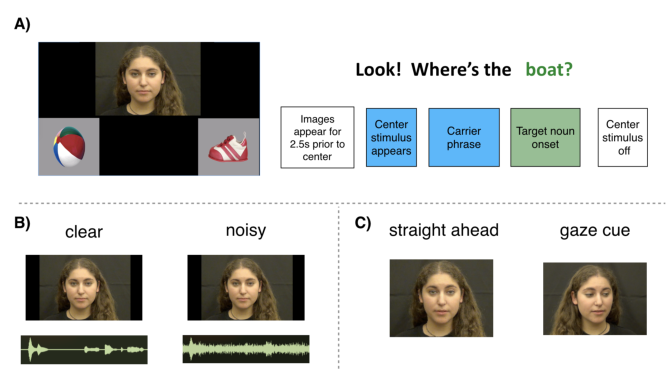
\includegraphics[width=0.8\linewidth]{figs/stimuli_plot-1} 

}

\caption[Stimuli information]{Stimuli information. Panel A shows the timecourse of the linguistic stimuli for a single trial. Panel B shows the layout of the three fixation locations (speaker, target, and distracter). And panel C shows a visual representation of the clear and noisy waveforms.}\label{fig:stimuli_plot}
\end{figure*}
\end{CodeChunk}

Here, we synthesize these ideas and test the generality of our
information-seeking account of eye movements during grounded language
comprehension. We ask whether listeners will adapt the timing of gaze
shifts away from a speaker if the auditory signal is less reliable -- as
is the case when processing speech in a noisy environment.

The second goal of this work is to test whether children would show a
similar pattern of behavior and flexibly adapt fixations in response to
changes in the utility of gathering certain kinds of visual information.
Recent developmental work shows that, like adults, preschoolers will
flexibly adjust how they interpret ambiguous sentences (e.g., ``I had
carrots and \emph{bees} for dinner.'') by integrating information about
the reliability of the incoming perceptual information with their
expectations about the speaker (Yurovsky, Case, \& Frank, 2017). While
children's behavior paralleled adults, they relied more on top-down
expectations about the speaker, perhaps because there was more inherent
perceptual noise for kids compared to adults. These developmental
differences provide insight into how children succeed in understanding
language despite having partial knowledge of word-object links and
without a fully-developed language model.

We hypothesized that a noisy auditory environment creates a scenario
where the auditory signal becomes less reliable, and in turn increases
the value of fixating on a speaker for the task of language
understanding. Our critical behavioral prediction is that listeners in
noisy contexts will delay generating an eye movement away from a speaker
until they have accumulated additional visual information about the
identity of the named referent. We also predicted that preschoolers
would show a parallel pattern of adaptation to noisy contexts and
allocate more fixations to a speaker's face when it became more useful
for accurate language comprehension.

To quantify evidence for our predictions, we analyze the Accuracy and
Reaction Times (RTs) of listeners' first gaze shifts after hearing the
name of an object in the visual scene. We focus on first shifts because
they provide a window onto changes in the underlying dynamics of
decision processes that generate eye movements. However, it is important
to point out that when we analyze differences in accuracy, we are not
making claims about the overall amount of time spent looking at the
target vs.~the distractor image -- a measure typically used in analyses
of the Visual World Paradigm.

\section{Experiment}\label{experiment}

In this experiment, we recorded adults and children's eye movements
during a real-time language comprehension task where participants
processed familiar sentences (e.g., ``Where's the ball?'') while looking
at a simplified visual world with three fixation targets (see Fig 1).
Using a within-participants design, we manipulated the signal-to-noise
ratio of the auditory signal by convolving the acoustic input with
Brownian noise (i.e., random noise patterns).

First, we present standard behavioral analyses of reaction time (RT) and
accuracy of listeners' first gaze shifts after target noun onset. Then,
we present two model-based analyses that link observable behavior to
underlying psychological constructs. We use an exponentially weighted
moving average (EWMA) method (Vandekerckhove \& Tuerlinckx, 2007) to
classify participants' gaze shifts as language-driven or random. In
contrast to the standard RT/accuracy analysis, the EMWA approach allows
us to quantify participants' willingness to generate gaze shifts after
noun onset but before collecting sufficient information to seek the
named referent. Higher values indicate that participants were waiting to
shift until they had accumulated enough of the linguistic signal to
locate the named referent. Finally, we use drift-diffusion models (DDMs)
(Ratcliff \& Childers, 2015) to ask whether behavioral differences in
accuracy and RT are driven by a more cautious responding strategy or by
more efficient information processing.

We predicted that processing speech in a noisy context would make
participants less likely to shift before collecting sufficient
information. This delay, in turn, would lead to a lower proportion of
shifts flagged as random/exploratory in the EWMA analysis, and a pattern
of DDM results indicating a prioritization of accuracy over and above
speed of responding (see the Analysis Plan section below for more
details on the models). We also predicted a developmental difference --
that children would produce a higher proportion of random shifts and
accumulate information less efficiently compared to adults -- and a
developmental parallel -- that children would show the same pattern of
adapting gaze patterns to gather more visual information in the noisy
processing context.

\subsection{Method}\label{method}

\subsubsection{Participants}\label{participants}

Participants were native, monolingual English-learning children (\(n=\)
39; 22 F, 17 M) and adults (\(n=\) 31; 22 F, 9 M). All participants had
no reported history of developmental or language delay and normal
vision. 14 participants (11 children, 3 adults) were run but not
included in the analysis because either the eye tracker falied to
calibrate (2 children, 3 adults) or the participant did not complete the
task (9 children).

\begin{CodeChunk}
\begin{figure*}[t]

{\centering 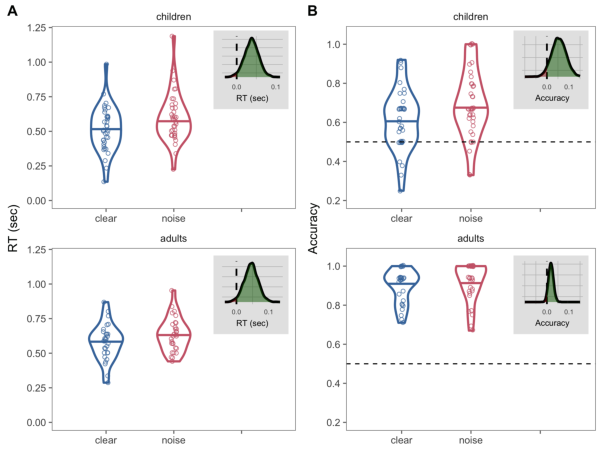
\includegraphics[width=0.9\linewidth]{figs/noise_acc_rt_e1_plot-1} 

}

\caption[Behavioral results for first shift Reaction Time (RT) and Accuracy]{Behavioral results for first shift Reaction Time (RT) and Accuracy. Panel A shows violin plots representing the distribution of RTs for each participant in each condition. Each point represents a participant's average RT. Color represents the processing context. The grey insets show the full posterior distribution of the plausible RT differences across conditions with the vertical dashed line representing the null value of zero condition difference. The green shading represents estimates in the predicted direction and above the null value while the red shading represents estimates below the null. Panel B shows the same information but for first shift accuracy.}\label{fig:noise_acc_rt_e1_plot}
\end{figure*}
\end{CodeChunk}

\subsubsection{Stimuli}\label{stimuli}

\emph{Linguistic stimuli.} The video/audio stimuli were recorded in a
sound-proof room and featured two female speakers who used natural
child-directed speech and said one of two phrases: ``Hey! Can you find
the (target word)'' or ``Look! Where's the (target word) -- see panel A
of Fig 1. The target words were: ball, bunny, boat, bottle, cookie,
juice, chicken, and shoe. The target words varied in length (shortest =
411.68 ms, longest = 779.62 ms) with an average length of 586.71 ms.

\emph{Noise manipulation}. To create the stimuli in the noise condition,
we convolved each recording with Brown noise using the Audacity audio
editor. The average signal-to-noise ratio\footnote{The ratio of signal
  power to the noise power, with values greater than 0 dB indicating
  more signal than noise.} in the noise condition was 2.87 dB compared
to the clear condition, which was 35.05 dB.

\emph{Visual stimuli.} The image set consisted of colorful digitized
pictures of objects presented in fixed pairs with no phonological
overlap between the target and the distractor image (cookie-bottle,
boat-juice, bunny-chicken, shoe-ball). The side of the target picture
was counterbalanced across trials.

\begin{CodeChunk}
\begin{figure}[t]

{\centering 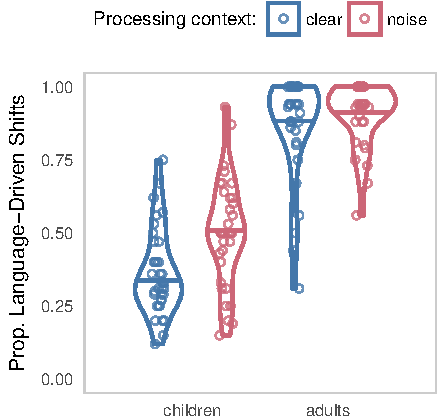
\includegraphics[width=0.8\linewidth]{figs/ewma_violin_plot-1} 

}

\caption[EWMA results for children and adults]{EWMA results for children and adults. Each point represents the proportion of shifts categorized as language-driven for a single participant. Color of represents the processing context: noise vs. clear.}\label{fig:ewma_violin_plot}
\end{figure}
\end{CodeChunk}

\begin{CodeChunk}
\begin{figure}[t]

{\centering 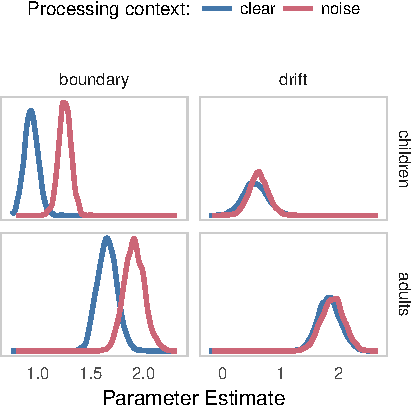
\includegraphics[width=0.8\linewidth]{figs/hddm_plot_noise-1} 

}

\caption[HDDM results]{HDDM results. Each panel shows the posterior distribution for either the boundary separation or drift rate parameters for children (top panels) and adults (bottom panels).}\label{fig:hddm_plot_noise}
\end{figure}
\end{CodeChunk}

\subsubsection{Design and procedure}\label{design-and-procedure}

Participants viewed the task on a screen while their gaze was tracked
using an SMI RED corneal-reflection eye-tracker mounted on an LCD
monitor, sampling at 60 Hz. The eye-tracker was first calibrated for
each participant using a 6-point calibration. On each trial,
participants saw two images of familiar objects on the screen for two
seconds before the center stimulus appeared (see Fig 1). Next, they
processed the target sentence -- which consisted of a carrier phrase, a
target noun, and a question -- followed by two seconds without language
to allow for a response. Child participants saw 32 trials (16 noise
trials; 16 clear trials) with several filler trials interspersed to
maintain interest. Adult participants saw 64 trials (32 noise; 32
clear). The noise manipulation was presented in a blocked design with
the order of block counterbalanced across participants.

\subsection{Analysis plan}\label{analysis-plan}

First, we present behavioral analyses of First Shift Accuracy and
Reaction Time (RT).\footnote{See \url{https://osf.io/g8h9r/} for a
  pre-registration of the analysis plan.} RT corresponds to the latency
to shift away from the central stimulus to either picture measured from
the onset of the target noun. (all RTs were analyzed in log space).
Accuracy corresponds to whether participants' first gaze shift landed on
the target or the distracter picture. We used the \texttt{rstanarm}
(Gabry \& Goodrich, 2016) package to fit Bayesian mixed-effects
regression models. The mixed-effects approach allowed us to model the
nested structure of our data -- multiple trials for each participant and
item, and a within-participants manipulation -- by including random
intercepts for each participant and item, and a random slope for each
item and noise condition. We used Bayesian estimation to quantify
uncertainty in our point estimates, which we communicate using a 95\%
Highest Density Interval (HDI). The HDI provides a range of credible
values given the data and model.

Next, we present the two model-based analyses -- the EWMA and DDM. The
goal of these models is to move beyond a description of the data and map
behavioral differences in eye movements to underlying psychological
variables. The EWMA method models changes in random shifting behavior as
a function of RT. For each RT, the model generates two values: a
``control statistic'' (CS, which captures the running average accuracy
of first shifts) and an ``upper control limit'' (UCL, which captures the
pre-defined limit of when accuracy would be categorized as above chance
level). Here, the CS is an expectation of random shifting to either the
target or the distracter image (nonlanguage-driven shifts), or a
Bernoulli process with probability of success 0.5. As RTs get slower, we
assume that participants have gathered more information and should
become more accurate, or a Bernoulli process with probability success
\textgreater{} 0.5. Using this model, we can quantify and compare the
proportion of gaze shifts that were likely to be language-driven as
opposed to random responding.

After we fit the EWMA, we took shifts categorized as language-driven and
fit a hierarchical Bayesian drift-diffusion model (HDDM). This model
quantifies differences in separable parameters of the underlying
decision process that lead to different patterns of behavior. The model
assumes that people accumulate noisy evidence in favor of one
alternative with a response generated when the evidence crosses a
pre-defined decision threshold. Here, we focus on two parameters of
interest: \textbf{boundary separation}, which indexes the amount of
evidence gathered before generating a response (higher values suggest
more cautious responding) and \textbf{drift rate}, which indexes the
amount of evidence accumulated per unit time (higher values suggest more
efficient processing).

\subsection{Results and Discussion}\label{results-and-discussion}

\subsubsection{Behavioral analyses:}\label{behavioral-analyses}

\textbf{RT.} To make RTs more suitable for modeling on a linear scale,
we analyzed responses in log space with the final model specified as:
\texttt{$log(RT) \sim noise\_condition + age\_group + (sub\_id + noise\_condition \mid item)$}.
Panel A of Figure 2 shows the full RT data distribution, the estimates
of condition means, and the full posterior distribution of the estimated
difference between the noise and clear conditions. Both children and
adults were slower to identify the target in the noise condition
(Children \(M_{noise}\) = 499.69 ms; Adult \(M_{noise}\) = 596.09 ms),
as compared to the clear condition (Children \(M_{clear}\) = 461.64 ms;
Adult \(M_{clear}\) = 550.9 ms). RTs in the noise condition were 41.73
ms slower on average, with a 95\% HDI ranging from 1.19 ms to 82.26 ms,
and not including the null value of zero condition difference.

\textbf{Accuracy.} Next, we modeled adults and children's first shift
accuracy using a mixed-effects logistic regression with the same
specifications (see Panel B of Fig 2). Both groups were more accurate
than a model of random responding (null value of \(0.5\) falling well
outside the lower bound of the 95\% HDI for all group means). Adults
were more accurate (\(M_{adults} =\) 90\%) than children
(\(M_{children} =\) 62\%). The key result is that both groups showed
evidence of higher accuracy in the noise condition: children
(\(M_{noise}\) = 67\%; \(M_{clear}\) = 62\%) and adults (\(M_{noise}\) =
92\%; \(M_{clear}\) = 90\%). Accuracy in the noise condition was on
average 4\% higher, with a 95\% HDI from 0\% to 11\%. Note that the null
value of zero difference falls at the very edge of the HDI such that
95\% of the credible values are greater than the null, providing
evidence for higher accuracy in the noise condition.

\subsubsection{Model-based analyses:}\label{model-based-analyses}

\textbf{EWMA.} Figure 3 shows the proportion of shifts that the model
classified as random vs.~language-driven for each age group and
processing context. On average, 41\% (95\% HDI: 32\%, 50\%) of
children's shifts were categorized as language-driven, which was
significantly less compared to adults, 87\% (95\% HDI: 78\%, 96\%).
Critically, processing speech in a noisy context caused both adults and
children to generate a higher proportion of language-driven shifts
(i.e., fewer random, exploratory shifts away from the speaker), with the
95\% HDI excluding the null value of zero condition difference
(\(\beta_{noise}\) = 12\%, {[}7\%, 17\%{]}). This pattern suggests that
the noise condition led participants to increase visual fixations to the
language source, leading them to generate fewer exploratory, random
shifts before accumulating sufficient information to respond accurately.

\textbf{HDDM.} Figure 4 shows the full posterior distributions for the
HDDM output. Children had lower drift rates (children \(M_{drift}\) =
0.58; adults \(M_{drift}\) = 1.9) and boundary separation estimates
(children \(M_{boundary}\) = 1.09; adults \(M_{boundary}\) = 1.67) as
compared to adults, suggesting that children were less efficient and
less cautious in their responding. The noise manipulation selectively
affected the boundary separation parameter, with higher estimates in the
noise condition for both age groups (\(\beta_{noise}\) = 0.27 {[}0.11,
0.42{]}). This result suggests that participants' in the noise condition
prioritized information accumulation over speed when generating an eye
movement in response to the incoming language. This increased decision
threshold led to higher accuracy. Moreover, the high overlap in
estimates of drift rate suggests that participants were able to
integrate the visual and auditory signals such that they could achieve a
level of processing efficiency comparable to the clear processing
context.

Taken together, the behavioral and EWMA/HDDM results provide converging
support for the predictions of our information-seeking account.
Processing speech in noise caused listeners to seek additional visual
information to support language comprehension. Moreover, we observed a
strikingly similar pattern of behavior in children and adults, with both
groups producing more language-driven shifts and prioritizing accuracy
over speed in the more challenging, noisy environment.

\section{General Discussion}\label{general-discussion}

Language comprehension in grounded contexts involves integrating
information from the visual and linguistic signals. But the value of
integrating visual information depends on the processing context. Here,
we presented a test of an information-seeking account of eye movements
during language processing: that listeners flexibly adapt gaze patterns
in response to the value of seeking visual information for accurate
language understanding. We showed that children and adults generate
slower but more accurate gaze shifts away from a speaker when processing
speech in a noisy context. Both groups showed evidence of prioritizing
information accumulation over speed (HDDM) while producing more
language-driven shifts (EWMA). Listeners were able to achieve higher
accuracy in the more challenging, noisy context. Together, these results
suggest that in settings with a degraded linguistic signal, listeners
support language comprehension by seeking additional language-relevant
information from the visual world.

These results synthesize ideas from several research programs, including
work on language-mediated visual attention (Tanenhaus et al., 1995),
goal-based accounts of vision during everyday tasks (Hayhoe \& Ballard,
2005), and work on effortful listening (Van Engen \& Peelle, 2014).
Moreover, our findings parallel recent work by McMurray, Farris-Trimble,
\& Rigler (2017) showing that individuals with Cochlear Implants, who
are consistently processing degraded auditory input, are more likely to
delay the process of lexical access as measured by slower gaze shifts to
named referents and fewer incorrect gaze shifts to phonological onset
competitors. McMurray et al. (2017) also found that they could replicate
these changes gaze patterns in adults with typical hearing by degrading
the auditory stimuli so that it shared features with the output of a
cochlear implant (noise-vocoded speech).

The results reported here also dovetail with recent developmental work
by Yurovsky et al. (2017). In their study, preschoolers, like adults,
were able to integrate top-down expectations about the kinds of things
speakers are likely to talk about with bottom-up cues from auditory
perception. Yurovsky et al. (2017) situated this finding within the
framework of modeling language as a \emph{noisy channel} where listeners
combine expectations with perceptual data and weight each based on its
reliability. Here, we found a similar developmental parallel in language
processing: that 3-5 year-olds, like adults, adapted their gaze patterns
to seek additional visual information when the auditory signal became
less reliable. This adaptation allowed listeners to generate more
accurate responses in the more challenging, noisy context.

This work has several important limitations that pave the way for future
work. First, we chose to focus on a single decision about visual
fixation to provide a window onto the dynamics of decision-making across
different language processing contexts. But our analysis does not
consider the rich information present in the gaze patterns that occur
leading up to this decision. In our future work, we aim to measure how
changes in the language environment might lead to shifts in the dynamics
of gaze across a wider timescale. For example, perhaps listeners gather
more information about the objects in the scene before the sentence in
anticipation of allocating more attention to the speaker once they start
to speak. Second, we chose one instantiation of a noisy processing
context -- random background noise. But we think our findings should
generalize to contexts where other kinds of noise -- e.g., uncertainty
over a speaker's reliability or processing accented speech -- shift the
priortization of gathering visual information to support language
understanding.

This experiment tested the generalizability of our information-seeking
account of eye movements within the domain of grounded language
comprehension. The account, however, is more general, and we are
interested in applying this framework -- an in-depth analysis of
decisions about visual fixation -- to the language acquisition context.
Consider that early in language learning, children are acquiring novel
word-object links while also learning about visual object categories.
Both of these tasks produce different goals that should, in turn,
modulate children's decisions about where to allocate visual attention
-- e.g., seeking nonlinguistic cues to reference such as eye gaze and
pointing become critical when you are unfamiliar with the information in
the linguistic signal. More generally, these results reflect a recent
theoretical emphasis on goal-based models of eye movements during
language comprehension (Salverda, Brown, \& Tanenhaus, 2011). We hope
that our approach is a way forward for explaining fixation behaviors
across a wider variety processing contexts and during different stages
of language learning.

\vspace{1em}
\fbox{\parbox[b][][c]{7.3cm}{\centering All data and code for this paper are available at\\url{https://github.com/kemacdonald/speed-acc/tree/master/paper/cogsci2018}}}
\vspace{1em}

\section{Acknowledgements}\label{acknowledgements}

We are grateful to the families who participated in this research.
Thanks to Tami Alade and Hannah Slater for help with data collection.
And thanks to Bria Long for helpful feedback on this paper. This work
was supported by an NSF GRFP to KM.

\section{References}\label{references}

\setlength{\parindent}{-0.1in} \setlength{\leftskip}{0.125in} \noindent

\hypertarget{refs}{}
\hypertarget{ref-allopenna1998tracking}{}
Allopenna, P. D., Magnuson, J. S., \& Tanenhaus, M. K. (1998). Tracking
the time course of spoken word recognition using eye movements: Evidence
for continuous mapping models. \emph{Journal of Memory and Language},
\emph{38}(4), 419--439.

\hypertarget{ref-erber1969interaction}{}
Erber, N. P. (1969). Interaction of audition and vision in the
recognition of oral speech stimuli. \emph{Journal of Speech and Hearing
Research}, \emph{12}(2), 423--425.

\hypertarget{ref-gabry2016rstanarm}{}
Gabry, J., \& Goodrich, B. (2016). Rstanarm: Bayesian applied regression
modeling via stan. r package version 2.10. 0.

\hypertarget{ref-hayhoe2005eye}{}
Hayhoe, M., \& Ballard, D. (2005). Eye movements in natural behavior.
\emph{Trends in Cognitive Sciences}, \emph{9}(4), 188--194.

\hypertarget{ref-macdonald1978visual}{}
MacDonald, J., \& McGurk, H. (1978). Visual influences on speech
perception processes. \emph{Attention, Perception, \& Psychophysics},
\emph{24}(3), 253--257.

\hypertarget{ref-macdonald2017info}{}
MacDonald, K., Blonder, A., Marchman, V. and, Fernald, A., \& Frank, M.
C. (2017). An information-seeking account of eye movements during spoken
and signed language comprehension. In \emph{Proceedings of the 39th
annual conference of the cognitive science society}.

\hypertarget{ref-macdonald2006constraint}{}
MacDonald, M. C., \& Seidenberg, M. S. (2006). Constraint satisfaction
accounts of lexical and sentence comprehension. \emph{Handbook of
Psycholinguistics}, \emph{2}, 581--611.

\hypertarget{ref-mcclelland2006there}{}
McClelland, J. L., Mirman, D., \& Holt, L. L. (2006). Are there
interactive processes in speech perception? \emph{Trends in Cognitive
Sciences}, \emph{10}(8), 363--369.

\hypertarget{ref-mcmurray2017waiting}{}
McMurray, B., Farris-Trimble, A., \& Rigler, H. (2017). Waiting for
lexical access: Cochlear implants or severely degraded input lead
listeners to process speech less incrementally. \emph{Cognition},
\emph{169}, 147--164.

\hypertarget{ref-ratcliff2015individual}{}
Ratcliff, R., \& Childers, R. (2015). Individual differences and fitting
methods for the two-choice diffusion model of decision making.
\emph{Decision}, \emph{2}(4), 237--279.

\hypertarget{ref-salverda2011goal}{}
Salverda, A. P., Brown, M., \& Tanenhaus, M. K. (2011). A goal-based
perspective on eye movements in visual world studies. \emph{Acta
Psychologica}, \emph{137}(2), 172--180.

\hypertarget{ref-smith2017multimodal}{}
Smith, A. C., Monaghan, P., \& Huettig, F. (2017). The multimodal nature
of spoken word processing in the visual world: Testing the predictions
of alternative models of multimodal integration. \emph{Journal of Memory
and Language}, \emph{93}, 276--303.

\hypertarget{ref-tanenhaus1995integration}{}
Tanenhaus, M. K., Spivey-Knowlton, M. J., Eberhard, K. M., \& Sedivy, J.
C. (1995). Integration of visual and linguistic information in spoken
language comprehension. \emph{Science}, \emph{268}(5217), 1632.

\hypertarget{ref-van2014listening}{}
Van Engen, K. J., \& Peelle, J. E. (2014). Listening effort and accented
speech. \emph{Frontiers in Human Neuroscience}, \emph{8}.

\hypertarget{ref-vandekerckhove2007fitting}{}
Vandekerckhove, J., \& Tuerlinckx, F. (2007). Fitting the ratcliff
diffusion model to experimental data. \emph{Psychonomic Bulletin \&
Review}, \emph{14}(6), 1011--1026.

\hypertarget{ref-yurovsky2017preschoolers}{}
Yurovsky, D., Case, S., \& Frank, M. C. (2017). Preschoolers flexibly
adapt to linguistic input in a noisy channel. \emph{Psychological
Science}, \emph{28}(1), 132--140.

\end{document}
